\label{section:3D_Example_Abdul}
These three examples simulate the fully three-dimensional surface/subsurface flows observed in  experiments conducted at Canadian Forces Base Borden, in Ontario, Canada, by Abdul (1985):
\begin{description}
    \item [Example 1 (\texttt{6\_Abdul\_Prism\_Cell)}:] A fully-coupled \gwf-\swf\ system receives recharge to the \swf\ domain and allows drainage from \swf\ cells located at the downstream outflow boundary.
        The template and \swf\ meshes are composed of 3-node triangular elements while the \gwf\ mesh is composed of 6-node prismatic elements.  The mesh-centred control volume approach is used to define the \mfus\ cells.
    \item [Example 2 (\texttt{\_Abdul\_Prism\_Cell\_nc}):] Similar to example 2 except the node-centred control volume approach is used to define the \mfus\ cells.
    \item [Example 3 (\texttt{6\_Abdul\_MODHMS}):] Similar to example 1 except The template and \swf\ meshes are composed of 4-node rectangular elements while the \gwf\ mesh is composed of 8-node hexahedral elements.
\end{description}

The following parameter values were used for the \gwf\ domain in all 3 examples:

\begin{center}
    \begin{tabular}{lll}  \hline
        Parameter                             & Value                       &     Unit                                \\ \hline
        Specific yield (porosity)             &  0.34                       &                   \\
        Hydraulic conductivity                &  $ 1 \times 10^{-5}$        &     m s$^{-1}$    \\
        Specific storage coefficient          &  $ 1.2 \times 10^{-7}$      &     m$^{-1}$      \\
        Van Genuchten Alpha                   &  1.9                        &     m$^{-1}$      \\
        Van Genuchten Beta                    &  6                          &                   \\
        Residual saturation                   &  0.18                     &                   \\
    \hline
    \end{tabular}
\end{center}

The Van Genuchten unsaturated function type was used.

For examples 1 and 2, the \swf\ domain was subdivided into 2 zones called grass and streambed as shown here for example 1:

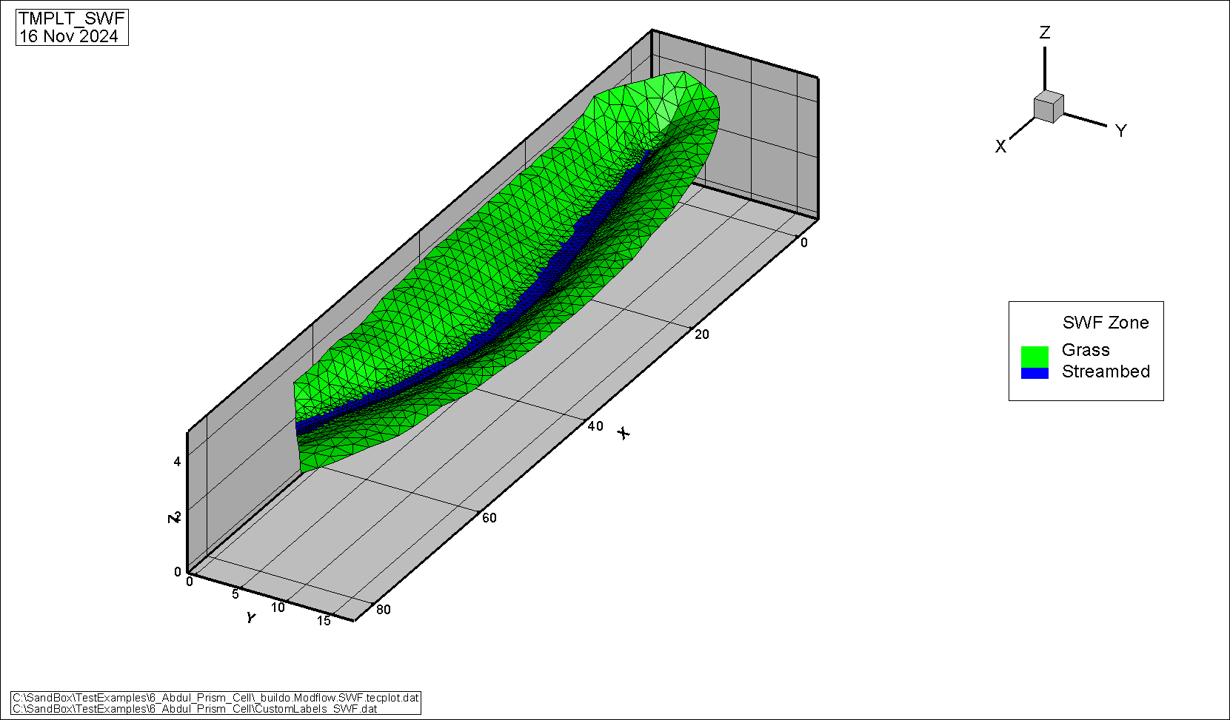
\includegraphics[width=0.7\textwidth]{5_7_SWFZones}

These parameter values were used for the grass zone for example 1 and 2:

\begin{center}
    \begin{tabular}{lll}  \hline
        Parameter                           & Value                         &   Unit            \\ \hline
        Manning's coefficient               &  0.3                          &   s m$^{-1/3}$   \\
        Depression storage height           &  0.1                          &   m               \\
        Obstruction storage height          &  0.0                          &   m               \\
        Depth for smoothing height 1        &  $1 \times 10^{-6}$     &   m               \\
        Depth for smoothing height 2        &  $1 \times 10^{-6}$     &   m               \\
    \hline
    \end{tabular}
\end{center}

These parameter values were calibrated and used for the streambed zone in examples 1 an 2:

\begin{center}
    \begin{tabular}{lll}  \hline
        Parameter                           & Value                         &   Unit            \\ \hline
        Manning's coefficient               &  0.01                         &   s m$^{-1/3}$   \\
        Depression storage height           &  0.1                          &   m               \\
        Obstruction storage height          &  0.0                          &   m               \\
        Depth for smoothing height 1        &  $3.75334 \times 10^{-3}$     &   m               \\
        Depth for smoothing height 2        &  $1.26394 \times 10^{-3}$     &   m               \\
    \hline
    \end{tabular}
\end{center}

Example 3 used a single \swf\ zone, which used these calibrated parameter values:

\begin{center}
    \begin{tabular}{lll}  \hline
        Parameter                           & Value                         &   Unit            \\ \hline
        Manning's coefficient               &  0.02                         &   s m$^{-1/3}$   \\
        Depression storage height           &  0.1                          &   m               \\
        Obstruction storage height          &  0.0                          &   m               \\
        Depth for smoothing height 1        &  $1.19106 \times 10^{-2}$     &   m               \\
        Depth for smoothing height 2        &  $2.49907 \times 10^{-2}$     &   m               \\
    \hline
    \end{tabular}
\end{center}

The 3 examples shared the following initial and boundary conditions:
\begin{itemize}
    \item An initial head of 2.78 m was assigned to the \gwf\ domain.
    \item An initial surface water depth of $1 \times 10^{-3}$  m was assigned to the \swf\ domain.
    \item A recharge of $5.56 \times 10^{-6}$ m/s was applied to the \swf\ domain for a time of 3000 s (stress period 1) then the recharge was reduced to 0.0 m/s for an additional 3000 s (stress period 2).
    \item A critical depth boundary was assigned to selected \swf\ cells located at the downstream end of the stream channel.
\end{itemize}

\pagebreak
Here is a comparison of measured and simulated stream outflow versus time for the Abdul field study.

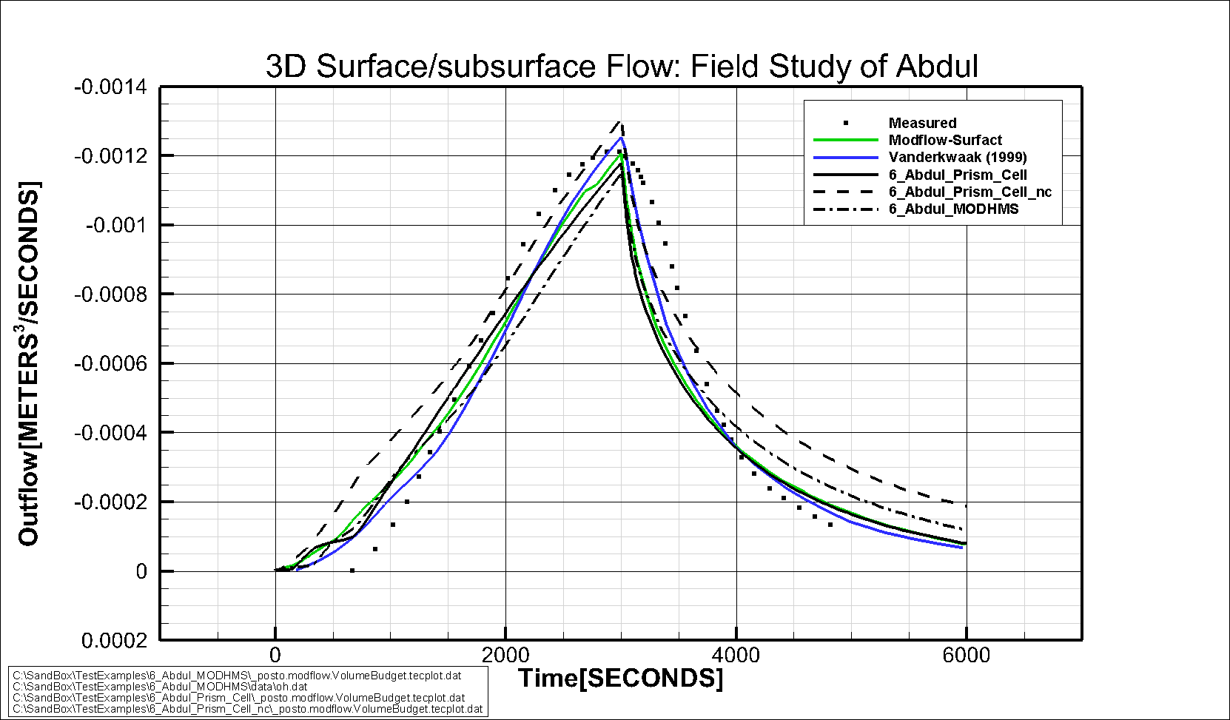
\includegraphics[width=0.87\textwidth]{5_8_Abdul_Outflow_3_Examples}

Simulation results are presented for the 3 examples as well as from \hgs\ and {\sc Modflow-Surfact}.  The results are similar for all cases.


